\documentclass[12pt]{article}
% Спільна преамбула для звітів (XeLaTeX)
\usepackage{fontspec}
\usepackage{polyglossia}
\setmainlanguage{ukrainian}
\setotherlanguage{english}
\setmainfont{DejaVuSerif}[Extension=.ttf,UprightFont=*,BoldFont=*-Bold,ItalicFont=*-Italic,BoldItalicFont=*-BoldItalic]
\setsansfont{DejaVuSans}[Extension=.ttf,UprightFont=*,BoldFont=*-Bold,ItalicFont=*-Oblique,BoldItalicFont=*-BoldOblique]
\setmonofont{DejaVuSansMono}[Extension=.ttf,UprightFont=*,BoldFont=*-Bold,ItalicFont=*-Oblique,BoldItalicFont=*-BoldOblique,Scale=0.9]
\usepackage[a4paper,margin=2.2cm]{geometry}
\usepackage{booktabs}
\usepackage{tabularx}
\usepackage{array}
\usepackage{enumitem}
\usepackage{xcolor}
\usepackage{tcolorbox}
\usepackage{graphicx}
\usepackage{setspace}
\usepackage[hidelinks]{hyperref}
\usepackage{titlesec}
\usepackage{fancyhdr}
\usepackage{multirow}
\usepackage{colortbl}
\setlength{\parskip}{4pt}
\setlength{\parindent}{0pt}
\onehalfspacing

\definecolor{accent}{HTML}{1F4E79}
\definecolor{sgreen}{HTML}{E2F0D9}
\definecolor{wred}{HTML}{FBE5D6}
\definecolor{oblue}{HTML}{DEEBF7}
\definecolor{tyellow}{HTML}{FFF2CC}
\definecolor{lightgray}{HTML}{F2F2F2}

\titleformat{\section}{\large\bfseries\color{accent}}{\thesection}{0.6em}{}
\titleformat{\subsection}{\normalsize\bfseries}{\thesubsection}{0.6em}{}

\pagestyle{fancy}
\fancyhf{}
\lhead{\small ІТ, Модуль 2 — командний проєкт}
\rhead{\small Петров Б., Мекшаков А.}
\cfoot{\thepage}
\renewcommand{\headrulewidth}{0.3pt}

\newcolumntype{L}[1]{>{\raggedright\arraybackslash}p{#1}}
\newcolumntype{Y}{>{\raggedright\arraybackslash}X}

% Титульна сторінка
\newcommand{\maketitlepage}[3]{%
\begin{titlepage}
\centering
{\large Київський національний університет імені Тараса Шевченка\\[2pt]
Факультет комп'ютерних наук та кібернетики\par}
\vspace{3cm}
{\large Дисципліна: \textbf{Інформаційні технології}\par}
\vspace{0.5cm}
{\large Модуль 2 — робота в команді\par}
\vspace{2cm}
{\LARGE\bfseries #1\par}
\vspace{0.6cm}
{\large #2\par}
\vfill
\begin{flushright}
\begin{tabular}{l}
\textbf{Виконали:} студенти 4 курсу, група МІ-41\\[4pt]
Петров Богдан\\
Мекшаков Артемій\\[10pt]
\textbf{Спеціальність:} Комп'ютерні науки\\
\end{tabular}
\end{flushright}
\vspace{1.5cm}
{Київ — #3\par}
\end{titlepage}
}

\usepackage{pdflscape}
\usepackage{float}

\begin{document}
\maketitlepage{Звіт за етапом 2}{Ініціація проєкту: Lean Canvas, карта продукту, простір проєкту}{2026}

\section{Мета етапу}
Остаточно затвердити тему командного проєкту з урахуванням результатів етапу~1, описати бізнес-модель продукту у форматі Lean Canvas, побудувати карту продукту (Product Roadmap) та створити простір проєкту на платформі управління командною роботою.

\section{Остаточно обрана тема}
За результатами SWOT-аналізу та зваженого порівняння трьох варіантів (етап~1) для розробки затверджено тему:

\begin{tcolorbox}[colback=oblue!40,colframe=accent,title=\textbf{StudyFlow --- планувальник навчальних дедлайнів для студентських груп}]
Вебзастосунок, що об'єднує в одному місці дедлайни, лабораторні та командні задачі навчальної групи: спільний календар, канбан-дошка, роль старости, e-mail-нагадування та прогрес групи.\\[4pt]
\textbf{Стек:} TypeScript, Next.js (frontend), NestJS (backend), PostgreSQL, Docker.\\
\textbf{Команда:} Петров Богдан (Team Lead, Backend), Мекшаков Артемій (Product Owner, Frontend, QA).
\end{tcolorbox}

Зміни відносно етапу~1: за результатами обговорення з викладачем тему прийнято без змін; уточнено, що канбан-дошка командних задач та e-mail-нагадування входять до обсягу семестру як функціонал другого пріоритету (Should), а інтеграції з Google Calendar / Classroom переносяться на наступні версії.

\newgeometry{margin=1.4cm,top=1.8cm}
\begin{landscape}
\section{Lean Canvas}\vspace{-6pt}
\renewcommand{\arraystretch}{1.0}\setlength{\tabcolsep}{4pt}
\footnotesize
\setlength{\extrarowheight}{0pt}
\begin{tabularx}{\linewidth}{|Y|Y|Y|Y|Y|}
\hline
\cellcolor{wred}\textbf{1. Проблема} & \cellcolor{tyellow}\textbf{4. Рішення} & \cellcolor{sgreen}\textbf{3. Унікальна ціннісна пропозиція} & \cellcolor{oblue}\textbf{9. Прихована перевага} & \cellcolor{lightgray}\textbf{2. Сегменти клієнтів}\\
\hline
\begin{itemize}[leftmargin=1em,nosep]
\item Дедлайни розпорошені між Classroom, чатами й усними домовленостями
\item Староста вручну дублює інформацію
\item Немає картини навантаження тижня
\end{itemize}
\textbf{Наявні альтернативи:} Google Calendar, Notion, Trello, чати в Telegram
&
\begin{itemize}[leftmargin=1em,nosep]
\item Групові дедлайни від старости --- один запис для всіх
\item Календар тижня/місяця з кольорами предметів
\item E-mail-нагадування за N днів
\item Канбан командних задач
\end{itemize}
&
\textbf{Один екран --- усі дедлайни групи.}

Створений старостою дедлайн миттєво з'являється у календарі кожного одногрупника, а нагадування приходять самі.

\textit{Концепт:} «Google Calendar, що знає, що таке група і староста»
&
\begin{itemize}[leftmargin=1em,nosep]
\item Спеціалізація на структурі навчання (предмет, група, староста)
\item Команда --- частина аудиторії, швидкий зворотний зв'язок
\item Мережевий ефект у межах групи
\end{itemize}
&
\begin{itemize}[leftmargin=1em,nosep]
\item Студенти університетів (18--24 роки)
\item Старости груп
\item Команди студентських проєктів
\end{itemize}
\textbf{Ранні послідовники:} група МІ-41 та сусідні групи факультету
\\
\cline{2-2}\cline{4-4}
& \cellcolor{tyellow}\textbf{8. Ключові метрики} & & \cellcolor{oblue}\textbf{5. Канали} & \\
\cline{2-2}\cline{4-4}
&
\begin{itemize}[leftmargin=1em,nosep]
\item Кількість активних груп і користувачів на тиждень (WAU)
\item Частка дедлайнів, виконаних вчасно
\item Кількість дедлайнів, створених старостою
\item Відкриття e-mail-нагадувань
\end{itemize}
& &
\begin{itemize}[leftmargin=1em,nosep]
\item Пряме впровадження через старост груп
\item Чати груп у Telegram
\item Рекомендації викладачів
\item Публічна demo-версія
\end{itemize}
& \\
\hline
\multicolumn{2}{|p{0.4\linewidth}|}{\cellcolor{wred}\textbf{7. Структура витрат}} & \multicolumn{3}{p{0.6\linewidth}|}{\cellcolor{sgreen}\textbf{6. Потоки доходів}}\\
\hline
\multicolumn{2}{|p{0.4\linewidth}|}{
\begin{itemize}[leftmargin=1em,nosep]
\item Час команди (два розробники, 4 спринти в семестрі)
\item Хостинг Vercel + Railway/Render, e-mail-сервіс (безкоштовні тарифи)
\end{itemize}} &
\multicolumn{3}{p{0.6\linewidth}|}{
\begin{itemize}[leftmargin=1em,nosep]
\item Базова версія безкоштовна для студентів (навчальний проєкт)
\item Потенційно: преміум для старост/груп (інтеграції, аналітика, Telegram-бот)
\item Потенційно: ліцензія для факультету/університету з адмін-панеллю
\end{itemize}}\\
\hline
\end{tabularx}
\end{landscape}
\restoregeometry

\section{Карта продукту (Product Roadmap)}
Карта продукту описує розвиток StudyFlow протягом одного року --- від прототипу в межах семестру до версії, придатної для впровадження на рівні факультету. Для кожного етапу визначено напрям розвитку, заплановані можливості та очікуваний результат.

\begin{table}[H]
\centering
\renewcommand{\arraystretch}{1.25}
\small
\begin{tabularx}{\textwidth}{L{2.4cm} L{2.6cm} Y Y}
\toprule
\textbf{Версія / період} & \textbf{Напрям} & \textbf{Заплановані можливості} & \textbf{Очікуваний результат}\\
\midrule
\textbf{MVP 0.1}\newline 28.10 -- 18.11.2026 & Ядро продукту &
Реєстрація та вхід; групи, інвайт-код, роль старости; предмети; особисті та групові дедлайни; список з фільтрами; календар тижня; відмітка виконання; Swagger; 20+ модульних тестів; E2E-тести; UML і схема БД &
Робочий прототип, який можна показати на захисті і дати спробувати групі МІ-41\\
\addlinespace
\textbf{0.2}\newline 19.11 -- 01.12.2026 & Стабілізація &
Канбан командних задач; e-mail-нагадування; календар місяця; прогрес групи; деплой demo-версії; фінальний звіт &
Публічна demo-версія; завершення модуля~2\\
\addlinespace
\textbf{1.0}\newline 12.2026 -- 02.2027 & Пілот і якість &
Пілотне використання в 2--3 групах; виправлення за зворотним зв'язком; відновлення пароля; налаштування нагадувань; особиста статистика; експорт iCal &
Стабільна версія з реальними користувачами; метрики WAU та частки вчасних дедлайнів\\
\addlinespace
\textbf{1.5}\newline 03.2027 -- 05.2027 & Інтеграції &
Імпорт із Google Classroom; синхронізація з Google Calendar; щотижневий дайджест; коментарі до задач &
Зниження ручного введення даних; утримання користувачів\\
\addlinespace
\textbf{2.0}\newline 06.2027 -- 08.2027 & Мобільність та канали &
PWA з push-сповіщеннями; Telegram-бот; графік навантаження групи &
Доступ з телефона; нагадування у звичних каналах\\
\addlinespace
\textbf{2.5}\newline 09.2027 -- 10.2027 & Масштабування &
Модель «факультет --- кілька груп»; адмін-панель; аналітика навантаження для викладачів; ретроспектива року &
Готовність до впровадження на рівні факультету\\
\bottomrule
\end{tabularx}
\caption{Карта продукту StudyFlow на рік}
\end{table}

\section{Простір проєкту на платформі управління}
Для управління задачами та командною роботою створено простір проєкту в \textbf{Notion} --- платформі, що поєднує базу задач, канбан-дошки та документацію проєкту в одному робочому просторі.

\subsection{Структура простору}
\begin{itemize}[leftmargin=1.5em]
  \item \textbf{Головна сторінка «StudyFlow --- командний проєкт»}: опис продукту, команда, ключові дати етапів, графік спринтів, правила роботи (гілки, pull request, Definition of Done).
  \item \textbf{База «StudyFlow --- Беклог»} (45 карток) з полями: ID, статус (Backlog / To Do / In Progress / Review / Done), тип (User Story / Tech / Docs), епік, пріоритет MoSCoW, квадрант матриці Ейзенхауера, спринт, виконавець, story points, опис.
  \item \textbf{Види бази:}
  \begin{itemize}[nosep]
    \item \emph{Kanban} --- дошка за статусом для щоденної роботи;
    \item \emph{Спринти} --- дошка за спринтами для планування та демо;
    \item \emph{Матриця Ейзенхауера} --- дошка за квадрантами важливості/терміновості;
    \item \emph{Таблиця} --- повний беклог із сортуванням за пріоритетом.
  \end{itemize}
\end{itemize}

\subsection{Процес роботи з дошкою}
Картка створюється у Backlog, під час планування спринта переходить у To~Do з призначеним виконавцем і спринтом; під час розробки --- In~Progress; після відкриття pull request --- Review (рев'ю виконує другий учасник); після злиття та проходження CI --- Done. Щотижневе демо проводиться за видом «Спринти».

\subsection{Демонстрація}
% Вставити скріншоти: головна сторінка, Kanban, вид «Спринти»
\begin{figure}[H]
\centering
\IfFileExists{img/notion-main.png}{
\includegraphics[width=0.8\textwidth,height=0.78\textheight,keepaspectratio]{img/notion-main.png}}{\fbox{\parbox{0.9\textwidth}{\centering\vspace{2cm}Скріншот: головна сторінка простору проєкту в Notion\vspace{2cm}}}}
\caption{Головна сторінка простору проєкту}
\end{figure}
\begin{figure}[H]
\centering
\IfFileExists{img/notion-kanban.png}{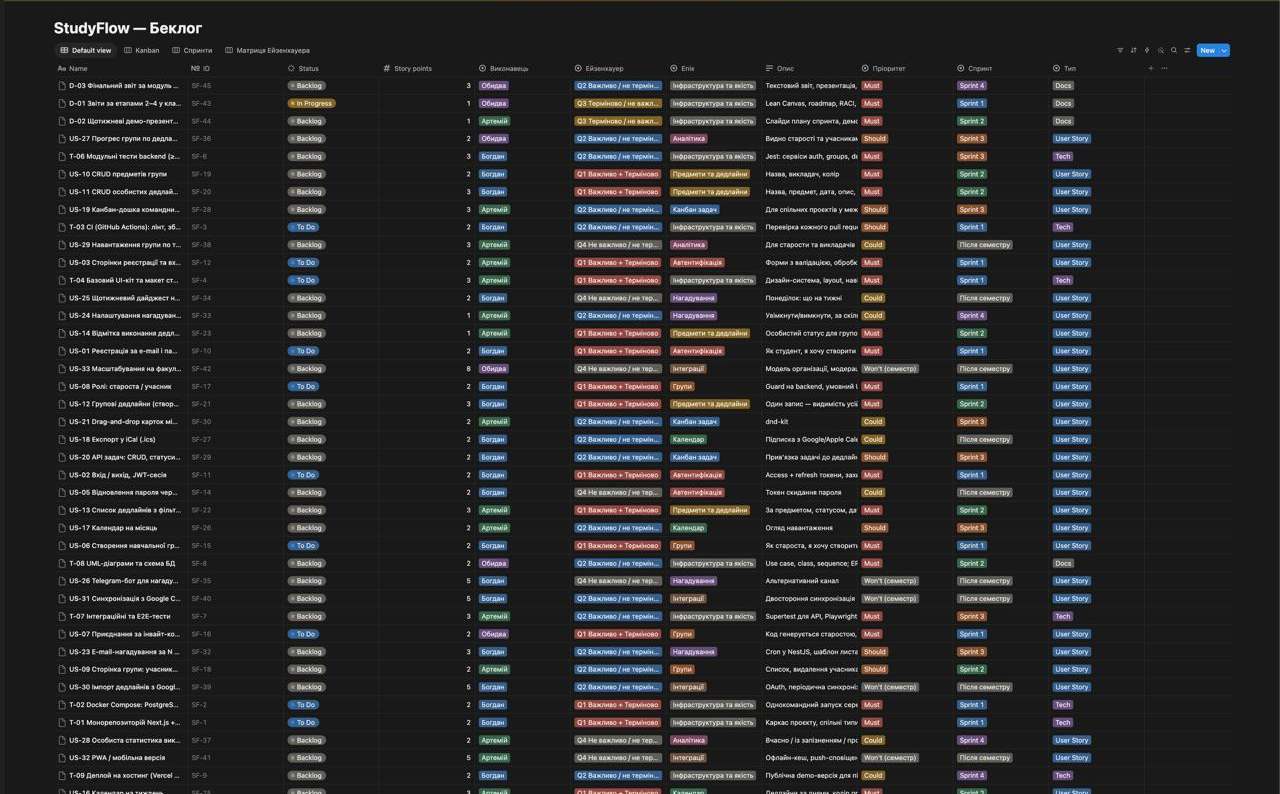
\includegraphics[width=0.95\textwidth,height=0.78\textheight,keepaspectratio]{img/notion-kanban.png}}{\fbox{\parbox{0.9\textwidth}{\centering\vspace{2cm}Скріншот: база беклогу\vspace{2cm}}}}
\caption{База «StudyFlow --- Беклог» (табличний вид; вкладки Kanban, Спринти, Матриця Ейзенхауера --- у верхній панелі)}
\end{figure}

\section{Результат етапу}
Тему StudyFlow остаточно затверджено; складено Lean Canvas, що фіксує проблему, сегменти, ціннісну пропозицію, канали, метрики та економіку продукту; побудовано карту продукту на рік із шістьма версіями; створено простір проєкту в Notion з беклогом із 45 карток і трьома канбан-видами. Наступний етап --- планування: дорожня карта з діаграмою Ґанта, RACI-матриця, пріоритезація беклогу та визначення обсягу семестру.

\end{document}
